\section{What is artificial intelligence?}
\setauthor{Romeo Bhuiyan}
The concept of \GLS{ai} has a long history that dates back to ancient times,
when people first tried to build machines that could mimic human abilities.
In the modern era, the term \textit{AI}  was first coined in 1956 by computer scientist 
John McCarthy, who defined it as \textit{the science and engineering of making 
intelligent machines} \footnote{johnmcCarthy:1956}.
% \cite[the science and engineering of making intelligent machines]{johnmcCarthy:1956} .

In modern times, advancements in technology have enabled machines to perform complex tasks such as speech recognition, 
decision-making, visual perception, and natural language understanding. These capabilities typically require human 
intelligence. The integration of AI into various industries, including healthcare, finance, 
education, and transportation, aims to enhance systems and improve their functionality. 
AI can be categorized into two primary types: strong or general AI and narrow or weak AI. 
Strong AI possesses the ability to perform any intellectual task that a human can, while narrow 
AI is designed for specific tasks and focuses on accomplishing a predefined objective. 
This distinction allows AI systems to address specific needs efficiently and effectively. \cite{KindsOfAI}

\subsection{AI in terms of Animotion}
\setauthor{Romeo Bhuiyan}
In the context of Animotion and their face and body tracking technology, AI refers to the utilization of Artificial Intelligence algorithms 
and techniques to enable accurate and efficient tracking of facial expressions and body movements.
Animotion employs AI algorithms to analyze and interpret visual data captured by camera or any ordinary webcam. These algorithms utilize machine learning and 
computer vision techniques to identify and track key facial landmarks and body poses in real-time. By analyzing the captured data, the 
AI algorithms can accurately determine the position, orientation, and movements of the face and body.
Through the power of AI, Animotion's technology can precisely track and analyze facial expressions and body movements, allowing for 
immersive experiences in applications such as virtual reality, augmented reality, gaming, and animation.

\section{Philosophy of artificial intelligence}
\setauthor{Christoph Lasinger}
Can a machine think? Thinking seems to be one of, if not the most important part of being human, as seen in René Descartes' 
first principle of philosophy “Cogito, ergo sum” (“I think, therefore I am”). So it goes to reason that, if we, as 
homo sapiens, were to see us superior to other animals on earth, it would be our intelligence, our conscious thinking, 
that would seem to differentiate us, make us special. Assuming this line of reasoning to be true, then it would only 
seem logical to think that we, as humans, are superior to machines in that regard as well. But what if that were to be taken away?

Throughout the course of history humans have practically been obsessed with self-imitation, be it wall-paintings, 
statues, portraits, photos, films or today's machines. The earliest example of artificial humans may be Greek gods, 
or rather Greek mythology as a whole, including for example architect and craftsman Daedalus, who created statues and 
machines that were sometimes impossible to distinguish from real human beings. Ancient Egypt also featured statues of 
gods behaving like humans and even though they were being controlled not by a god, but through complex mechanisms, 
such as quicksilver or hydraulics, or even simple puppeteering strings, the Egyptians still feared and revered them. 
They saw it not as blasphemy but as gods acting through guided souls, even though they might be that of a master and puppet.

However, not everyone would view such creations as positive as the Greeks and Egyptians. As even before their 
time a different culture, or to be more accurate religion had rules regarding artificial humans, the so called 
ten commandments, of which the second one states “You shall not make for yourself a carved image, or any likeness 
of anything that is in heaven above, or that is in the earth beneath, or that is in the water under the earth. 
You shall not bow down to them or serve them, for I the Lord your God am a jealous God ...". Of course, any religious 
text is open to interpretation, but it seems a rather popular one was that of Hermes Trismegistor, purported author 
of the Hermetica, a series of ancient texts that lay the basis of philosophical systems known as Hermetecicism, 
who stated that man has created statues, infused with the souls of demons and angels through holy rituals.

The purpose of mentioning these two views regarding artificial humans is that they are essentially the 
two fundamental views of the western world regarding “thinking machines”, or artificial intelligence, 
as well. This can be seen in statements made by both critics and proponents of AI. \cite{Denkmaschinen}
\newpage
\section{The future of artificial intelligence}
\setauthor{Romeo Bhuiyan}

Predicting the future of AI is challenging, but it is highly probable that AI will continue its advancement and 
integration into various aspects of our daily lives. This technology holds the potential to revolutionize numerous 
industries, including healthcare, transportation, education, and finance. As AI progresses, it may automate certain 
jobs while creating new ones to support its implementation. However, it is crucial to address ethical considerations 
to ensure responsible development and use of AI. While the future of AI appears promising, it necessitates a cautious 
and thoughtful approach. It is prudent to analyze both extreme optimism and extreme pessimism scenarios to gain a 
comprehensive understanding of AI's potential outcomes.

Extreme pessimism regarding the future of AI entails a vision where AI technology supplants human jobs, 
resulting in extensive unemployment and socioeconomic disruption. The impact on IT jobs is often emphasized, 
specifically regarding the potential displacement of customer service representatives, chat agents, and support 
personnel by AI-powered chatbots and virtual assistants. AI's ability to automate routine IT tasks like system monitoring 
and data analysis further contributes to concerns. However, it is essential to consider the potential for job creation and 
transformation, such as AI system development, algorithm design, and AI ethics roles. Additionally, human-centric skills 
involving critical thinking, creativity, and complex decision-making remain integral to IT professions. Reskilling and upskilling 
initiatives are vital to mitigate job displacement, empowering individuals to adapt to the evolving AI-driven workforce 
by acquiring interdisciplinary skills.

Extreme optimism about AI's future involves a harmonious partnership between AI technology and human 
professionals, leading to increased productivity and positive outcomes in IT jobs. ChatGPT and similar 
conversational AI models have potential in revolutionizing customer service and support roles by offering 
personalized interactions and empowering human agents. AI significantly contributes to task automation in IT, 
streamlining processes such as software testing and system monitoring. This automation allows IT professionals to 
focus on strategic initiatives, optimizing network management and reducing costs. The integration of AI creates new 
opportunities for roles like AI system developers, data scientists, and AI ethics professionals. Human skills like critical 
thinking and problem-solving remain essential, with AI acting as a powerful tool to augment human capabilities in delivering high-quality solutions.

\section{The functional concept of neural networks}
\setauthor{Romeo Bhuiyan}
A neuronal network is a type of machine learning algorithm modeled 
after the structure and function of a human brain (neural linking). 
It is composed of many interconnected processing nodes, called neurons, 
which work together to process information. 
\\
\begin{figure}[htb]
    \centering
    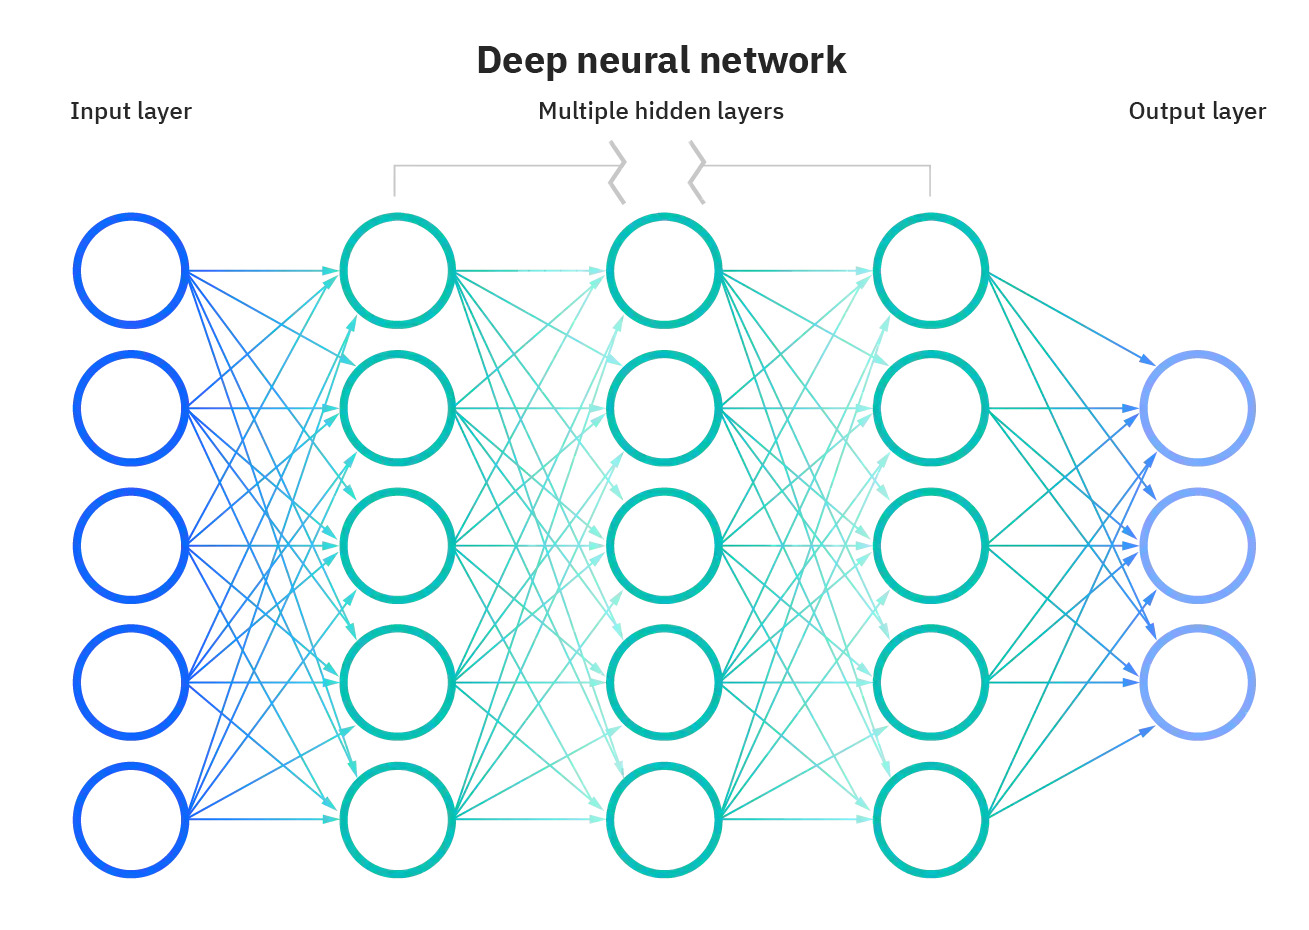
\includegraphics[width=0.8\textwidth]{pics/neuralnetwork.jpg}
    \caption{Complex neural network}
    \label{fig:neuralnetwork}
    \cite{IBM}
\end{figure}
\\
As shown in figure \ref{fig:neuralnetwork}, each neuron receives input from other neurons, processes that information, 
and produces an output. This output is then passed on to other neurons in the next 
layer of the network. In this way, information is passed through the network, from the 
input layer to the output layer, allowing the neural network to learn and make predictions
based on the data it is given. \cite{book1}

The specifics of how a neural network works can vary depending on its architecture and the type of problem it is used to solve. 
However, in general, a neural network can learn from data by adjusting the strength of the connections between its neurons, which 
are called weights, based on the input it receives. Over time, the network can improve its predictions by adjusting these weights 
to minimize errors between the network output and the correct output. These weights may vary depending on the type of AI being used. In the case of Animotion, the most important weights for face 
tracking are related to facial features such as the eyes, nose, and mouth. The weights associated with these features determine 
the shape of the mouth and the movement of the pupils of the eyes.
Another important weight for motion tracking in Animotion is motion dynamics, 
which refers to the facial and body movements that contribute to a smoother 
user experience. These weights are vital for enabling the neural network to 
learn and recognize patterns and variations in motion, resulting in more 
natural and realistic tracking.

However, it is important to note that certain weights may not be 
applicable when working with input obtained via a webcam. In this 
case, factors such as depth and distance, which are crucial for 
capturing accurate three-dimensional information, may pose 
challenges. Estimating the depth of different facial or 
body parts is essential for understanding spatial relationships 
and achieving realistic motion representation. Achieving a balance between maintaining accuracy and obtaining 
a satisfactory output requires careful consideration and 
optimization of the other weights in the AI system. By carefully adjusting and fine-tuning the weights associated 
with motion dynamics, facial features and other relevant factors, 
the Animotion AI network can optimize its tracking capabilities 
and provide a compelling user experience while accounting for the 
limitations of webcam-based input. \cite{weights}

\subsection{Solving methods}
There are three basic methods for solving problems: 
search-, knowledge-, and algorithmic methods. 
Every method involves searching through a space of possible
solutions whilst optimizing a pre-defined evaluation function, 
that can lead to the following \emph{Combinatorial explosion} as shown below in the figure \ref{fig:combiexplo}. 
The methods can range from \emph{simplex hill climbing via alpha-beta pruning techniques} to \emph{knowledge chunking}. 

\textbf{Simplex hill climbing via alpha-beta pruning techniques} is a combination of two different methods used to solve optimization problems 
in artificial intelligence. Simplex hill climbing is an iterative method that tries to find the maximum or minimum value of an objective function 
by repeatedly changing the input values and evaluating the function at each point until a peak or valley is found. The alpha-beta pruning 
technique is a search algorithm used in game theory to reduce the number of nodes evaluated in a minimax algorithm.

The simplex hill climbing algorithm starts with a randomly selected point in the search space and then moves to the neighboring points 
in each iteration, depending on the function's value at that point. The goal is to eventually reach the point that maximizes or minimizes 
the function, depending on the problem's objective. However, this method can be slow, especially for higher-dimensional search spaces, 
as the search may get stuck in a local maximum or minimum that is not the global optimum. To speed up the search process, the alpha-beta 
pruning technique can be applied. This technique uses a cutoff mechanism to eliminate 
parts of the search tree that cannot influence the final result. By pruning the tree, the search algorithm can avoid evaluating nodes 
that are unlikely to lead to a better solution, reducing the number of evaluations required to find the optimal solution. This approach 
is particularly useful for search spaces with many branches, such as game trees.

By combining these two techniques, simplex hill climbing via alpha-beta pruning can efficiently and effectively search for optimal 
solutions in complex optimization problems. The algorithm is particularly useful for problems that have large search spaces or are 
difficult to solve with other methods. However, like any algorithm, it has its limitations and may not always be the best choice 
for every problem. \cite{pruning}

\textbf{Knowledge chunking} is a technique used in artificial intelligence to improve problem-solving efficiency by breaking down complex problems 
into smaller, more manageable parts or \emph{chunks}. The process of chunking involves identifying patterns and relationships within a problem 
and grouping similar elements together into chunks. These chunks are then treated as separate entities, allowing for more efficient processing and retrieval from memory.

This has been shown to be effective in a range of AI applications, including natural language processing, expert systems, 
and machine learning. By breaking down complex problems into smaller, more manageable pieces, knowledge chunking allows AI systems to 
more effectively reason, learn, and make decisions. Additionally, the use of chunking can improve the scalability and generalizability 
of AI systems by allowing them to better handle larger, more complex datasets. Overall, knowledge chunking is a valuable technique for 
improving the efficiency and effectiveness of AI systems across a range of applications. \cite{knowledgechunking}

Example: the chess endgame of king and three pawns versus king 
and three pawns requires an explicit table of half a billion 
moves and a run-time of ten quadrillion years to evaluate all
possibilities. The success of the cmu chunker programm which
uses chess domain knowledge chunks is that it reduces this
run-time to about one minute.
\\
\begin{figure}[htb]
    \centering
    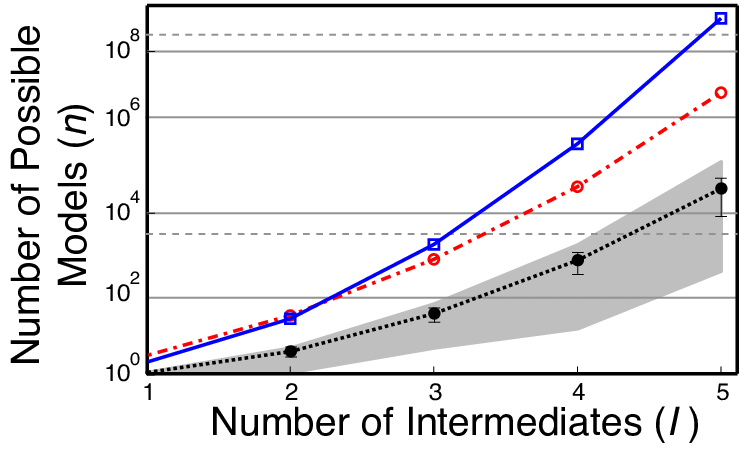
\includegraphics[width=0.5\textwidth]{pics/combiexplo.png}
    \caption{Combinatorial explosion} 
    \cite{combiexplo}
    \label{fig:combiexplo}
\end{figure}
\\
\newpage
\subsection{Landmark-Tracking}
\setauthor{Romeo Bhuiyan}
Regarding Animotion \textbf{Landmark-Tracking} was used and the first step is to detect
and locate the face in an image or video frame. 
This can be achieved using algorithms like Haar cascades, 
Histogram of Oriented Gradients, or more advanced 
techniques. In this case Haar cascades were used which was also
used for face detection. It involves training a classifier with positive 
and negative samples to identify patterns in an image. By applying a 
series of Haar-like features, as shown in the figure below \ref{fig:haarcascade}, it efficiently filters out non-face 
regions and quickly detects potential face regions. It is widely 
used for real-time face detection applications. \cite{landmarks}
\\
\begin{figure}[htb]
    \centering
    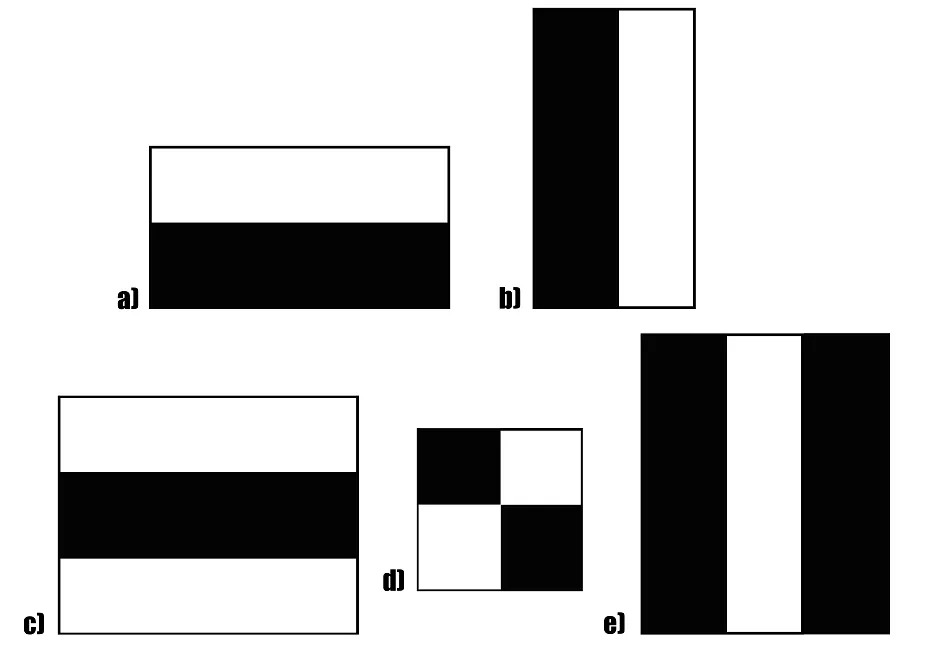
\includegraphics[width=0.5\textwidth]{pics/haarlike.jpg}
    \caption{Haar-like features are simple rectangular areas used in computer vision algorithms, 
    particularly in face detection. These features capture variations in pixel intensities within 
    different regions of an image. They are named after Alfred Haar, a mathematician who introduced them.
    (Original image used in the research paper \emph{Rapid Object Detection using a Boosted Cascade of Simple
    Features} by Viola and Jones)}
    \cite{haarcascade}
    \label{fig:haarcascade}
\end{figure}
\\
Once the face is detected, the next step is to identify key facial landmarks 
such as the eyes, nose, mouth, and other distinctive points. These landmarks 
provide important reference points for tracking facial movements. The Method
\emph{Active Shape Models (ASM)} deep learning-based facial landmark detector was used for this purpose.
It is a model-based approach that utilizes a predefined model to find the 
optimal alignment between the model and new image data. By comparing the 
model with the data, it attempts to locate the best match position. Once 
the model is aligned, measurements can be made to determine the presence 
of the target object. \cite{ASM}

After detecting the initial set of facial landmarks as shown in the figure below \ref{fig:facetracking}, 
a tracking algorithm is employed to follow the movement of these landmarks over time.
Various tracking algorithms can be used but the decision has been made on the Kanade-Lucas-Tomasi (KLT) tracker, named after
the inventors Kanade, Lucas and Tomasi who came up with a Method for tracking an image patch and Method for choosing the
best feature on this image for tracking. The KLT tracker follows these landmarks by estimating the motion of each 
landmark from frame to frame. It does this by assuming that the motion of each landmark is relatively small between 
successive frames.

The KLT tracker operates based on two main principles: \textbf{feature tracking} and \textbf{feature selection}. 
In \textbf{feature tracking}, the algorithm searches for the corresponding location of each landmark in the 
subsequent frame by analyzing the local image region surrounding the landmark. It uses the brightness 
constancy assumption, which states that the intensity pattern of a landmark remains unchanged between frames, 
to estimate its new position.
Once the potential locations of the landmarks are determined in the subsequent frame, the KLT tracker applies 
the Lucas-Kanade algorithm to calculate the optical flow, which represents the motion vector of each landmark. 
The algorithm uses a small patch around each landmark and iteratively refines the motion estimation by minimizing 
the intensity difference between the patch in the current frame and its corresponding patch in the previous frame.
To ensure robust tracking, the KLT tracker employs \textbf{feature selection}. 
It chooses the best features among the detected landmarks based on their quality and reliability. 
The Harris corner detection algorithm was used for fine-tuning and to evaluate the quality of each feature. 
The features with higher quality are considered more distinctive and suitable for tracking.

\begin{figure}[htb]
    \centering
    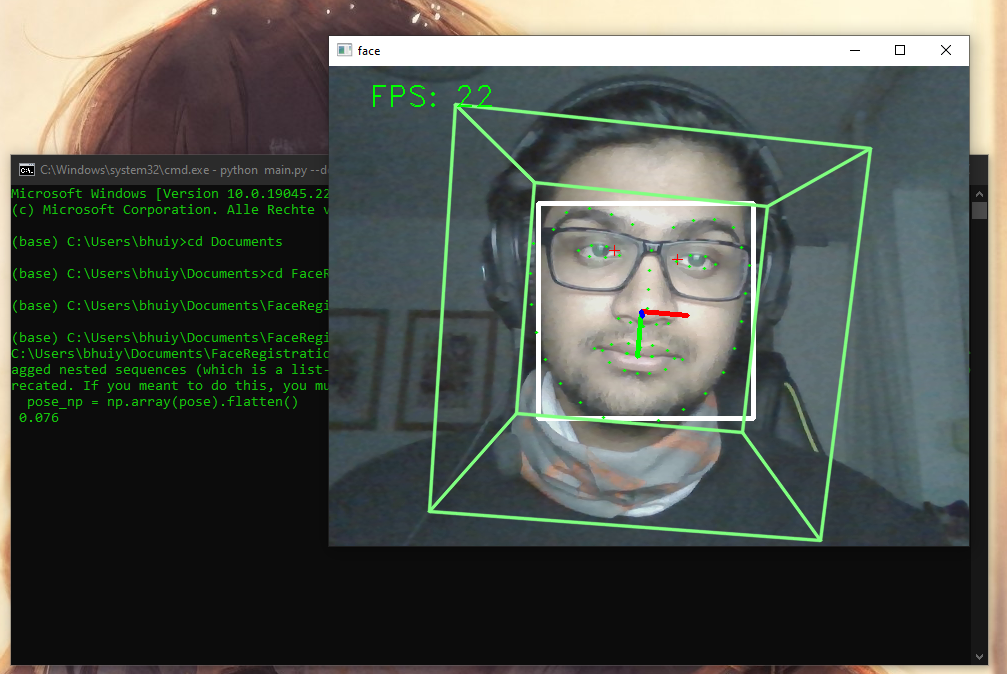
\includegraphics[width=0.8\textwidth]{pics/bhuiyanfracetracking.png}
    \caption{Face detection and tracking done by Romeo Bhuiyan}
    \label{fig:facetracking}
\end{figure}

\subsection{Harris corner detection algorithm }
\setauthor{Romeo Bhuiyan}
The Harris corner detection algorithm, introduced by Chris Harris and Mike Stephens in 1988, is widely 
employed for detecting corners or key points in images. It has become a popular choice in computer vision and 
image processing applications, such as feature detection, image matching, and object recognition.
This algorithm identifies corners by leveraging the observation that corners are areas in an image where the 
intensity gradient exhibits notable variations in multiple directions. By examining every pixel in an image, the 
algorithm computes a corner score that reflects the local intensity variations. \cite{harristheory2}

\subsubsection{How it works}
Beginning with the preprocessing step, the input image is converted to grayscale, 
unless it is already in grayscale. Grayscale images are commonly preferred for corner detection 
since the detection process relies on analyzing intensity variations.

After that the Harris corner detection algorithm involves computing the gradients of the image. 
This is accomplished by applying a suitable gradient operator, such as the Sobel operator. 
The purpose of calculating these gradients is to determine the intensity changes that occur in 
both the horizontal and vertical directions at each pixel. By analyzing the gradient values, the 
algorithm gains insight into the image's local intensity variations, which is crucial for 
accurately identifying corners or key points.

The next step involves calculating the structure tensor. This tensor is a matrix that encapsulates 
the local intensity variations for each pixel in the image. To compute the structure tensor, the algorithm 
considers a small neighborhood around the pixel and calculates the sum of the products of the gradients within 
that region. By aggregating this information, the structure tensor provides insights into the image's local 
characteristics, enabling the algorithm to effectively detect corners and key points.

Then the following step is to calculate the corner response function. This function serves as a measure of the likelihood that a pixel represents a corner. 
In the Harris corner detection algorithm, the corner response function is defined as
\begin{equation}
    \label{eqn:harris}
    R = det(M) - k \cdot trace(M)^2
\end{equation}
where M represents the structure tensor.
To derive the corner response function, two key components of the structure tensor, the determinant \emph{(det(M)) and the trace (trace(M))}, are used. 
The determinant provides information about the tensor's overall characteristics, while the trace represents the sum of the tensor's diagonal elements.
The constant \emph{k} in the equation is typically determined empirically.
By evaluating the corner response function for each pixel in the image, higher response values indicate a higher likelihood 
of the pixel being a corner. This response function plays a crucial role in the subsequent steps of corner detection, where a threshold is 
applied to select pixels with significant corner responses and eliminate those with lower values. What this resulted in, is shown in the figure below \ref{fig:harriscorner}.

The Harris corner detection algorithm includes two more steps at the end: thresholding and non-maximum suppression.
Firstly, thresholding is used to select pixels with high corner scores by setting a certain limit. 
This helps identify important corners while ignoring less important ones.
Next, non-maximum suppression is applied to handle situations where multiple corner points are very close to each other. 
This step ensures that only the most prominent corner points are kept in the final result. By removing redundant corner points, 
non-maximum suppression improves the accuracy of corner detection and reduces the chances of detecting the same corner multiple times. \cite{harristheory} \cite{harrisworks}
\\
\begin{figure}[htb]
    \centering
    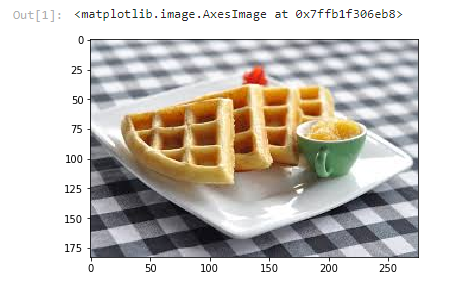
\includegraphics[width=0.4\textwidth]{pics/HarrisWaffle.png}
    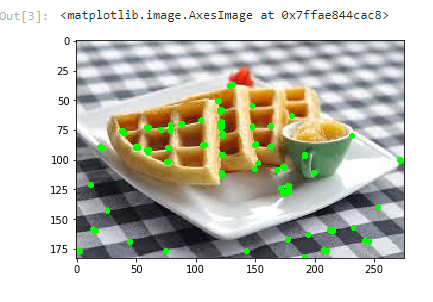
\includegraphics[width=0.4\textwidth]{pics/HarrisWaffle2.png}
    \caption{Getting the corners of a waffle with the Harris corner detection algorithm}
    \label{fig:harriscorner}
    \cite{waffleimage}
\end{figure}
\\

\section{Comparison of machine learning frameworks}
\setauthor{Romeo Bhuiyan}
In this case face tracking was needed in order to get a virtual model animated. 
The two libraries MediaPipe and TensorFlow.js were tested using python to decide 
which one is better suited for our purpose. It is difficult to say which approach 
is more suitable for face, hand, and body tracking in the browser, as it will depend 
on the specific requirements and constraints of one's project. Both MediaPipe and 
TensorFlow.js are powerful tools that can be used to perform these tracking tasks, 
but they have different strengths and limitations.

\textbf{MediaPipe} is a library developed by Google that is specifically designed 
for real-time multimedia processing tasks, such as hand and face tracking. 
It is written in C++ with some Python bindings and can be used to build cross-platform 
pipelines for performing various computer vision and machine learning tasks. MediaPipe is 
optimized for low-latency, real-time processing and is used to build applications that run 
on a variety of platforms, including the browser. \cite{Mediapipe}

In contrast, \textbf{TensorFlow.js} is a JavaScript library for training and deploying machine 
learning models in the browser. It is based on the TensorFlow library, a popular machine 
learning library developed by Google. TensorFlow.js allows you to build and train machine 
learning models using JavaScript, and it can be used to perform a variety of tasks, including 
image and text classification, time series forecasting, and natural language processing. \cite{Tensorflow}

In \textbf{Conclusion}, both MediaPipe and TensorFlow.js are able to handle face and hand
tracking in the browser, but personal experiments were conducted based on connectivity with the VRM model rigging in order to find out 
that they have different trade-offs and may be better suited
for different types of projects. MediaPipe is optimized for real-time processing and is
good for building applications that require low latency, such as augmented reality or
interactive applications. However, TensorFlow.js is a general-purpose machine learning
library that is suited for building machine learning models and deploying them in the
browser, but it may not be as efficient for real-time processing as MediaPipe. 
At the end of the Python experiment, the camera controls worked better with only one of these libraries, 
and thinking that more content will likely be added to the project in the future, it has been decided 
to use MediaPipe as our real-time multimedia library solution.

\section{Optimizing artificial intelligence models through training}
\setauthor{Romeo Bhuiyan}
AI training plays a pivotal role in the development of AI systems. It entails inputting substantial data into an AI model to facilitate 
its accurate learning and task performance. The effectiveness of the AI system depends on the quality of the training data 
and the algorithms utilized during the training process.
The significance of AI training lies in its capacity to establish a foundation for smarter and more capable AI systems. 
These systems can adeptly handle complex tasks with a high level of accuracy. AI training enables systems to make predictions, 
process vast amounts of data, and automate tasks, thereby enhancing their efficiency and effectiveness.
For instance, AI training is leveraged in natural language processing to teach models how to comprehend and respond 
to human speech. In computer vision, it trains models to recognize and categorize images and objects. Additionally, 
in robotics, AI training equips models with the ability to navigate and perform physical tasks.\cite{training}

Animotion utilized a specific training procedure to enhance the performance of their AI system. 
The procedure involved several steps aimed at achieving smooth tracking and realistic transfer to a 3D model.
To begin with, the AI system was kept continuously operational without any reboots. 
This ensured the system's stability and allowed for uninterrupted training.
A human subject was then positioned in front of the AI system, and a series of gestures were performed. 
These gestures served as the input data for the training process. By observing and analyzing these gestures, 
the AI system learned to track and accurately capture the movements in real-time.
Through an iterative process of training and fine-tuning, the AI system gradually improved its tracking capabilities.
Parameters and algorithms were adjusted to optimize the tracking performance based on the observed gestures. 
This iterative training approach allowed the system to adapt and improve its accuracy over time.
Once the training phase was completed, the acquired knowledge from tracking the gestures was transferred to a 3D model. 
This transfer involved mapping the tracked gestures onto the corresponding movements of the 3D model, ensuring synchronized animation.
One of the primary goals of this training procedure was to achieve smooth animation. By continuously training the 
AI system with a diverse range of gestures, Animotion refined the tracking and transfer process. 
This refinement resulted in animations that appeared seamless and lifelike, closely resembling the original gestures performed by the human subject.

\subsection{Anaconda}
\setauthor{Romeo Bhuiyan}
Anaconda is a widely used software distribution platform that focuses on managing and deploying 
data science tools and libraries for the Python programming language. It provides a comprehensive environment 
for data analysis, scientific computing, and machine learning. \cite{anaconda}
Animotion, utilizes Anaconda as part of their development process to refine their face tracking system. 
Specifically, they employ Anaconda to facilitate the fine-tuning of their face tracking algorithm 
using the Harris corner detection algorithm.
By leveraging Anaconda's extensive range of data science tools and libraries, Animotion can 
efficiently adjust and optimize the parameters and configurations of their face tracking algorithm. 
This iterative fine-tuning process allows them to enhance the accuracy and performance of their face tracking system, 
ensuring more precise and reliable tracking results as shown in the listing below \ref{lst:detectionbox}. 

\begin{lstlisting}[language=Python,caption=detecting the face in a box shaped object,label=lst:detectionbox]
    def get_face(detector, image, cpu=False):
    if cpu:
        image = cv2.cvtColor(image, cv2.COLOR_BGR2GRAY)
        try:
            box = detector(image)[0]
            x1 = box.left()
            y1 = box.top()
            x2 = box.right()
            y2 = box.bottom()
            return [x1, y1, x2, y2]
        except:
            return None
    else:
        image = cv2.resize(image, None, fx=0.5, fy=0.5)
        box = detector.detect_from_image(image)[0]
        if box is None:
            return None
        return (2 * box[:4]).astype(int)
\end{lstlisting}

The provided code above \ref{lst:detectionbox} defines a function called \texttt{get\_face} that is used to extract the coordinates of a detected face within an image. 
The function takes three parameters: \texttt{detector, image, and cpu}.
The purpose of this function is to leverage a face detection algorithm provided 
by the \emph{harris corner} detection \emph{algorithm} object and apply it to the input image in order to identify 
and locate faces within the image. The code includes two different branches of execution based on the value of the \texttt{cpu} flag.
If \texttt{cpu} is set to \texttt{True}, the face detection is performed on the CPU. 
In this case, the image is first converted to grayscale using the OpenCV function \texttt{cv2.cvtColor()}. 
The face detection algorithm, assumed to be encapsulated within the \texttt{detector} object, is then applied to the grayscale image. 
The resulting bounding box of the detected face is obtained, and its coordinates (\texttt{left, top, right, bottom}) are extracted. 
These coordinates represent the top-left and bottom-right points of the bounding box. Finally, the coordinates are returned as a list \texttt{[x1, y1, x2, y2]}.

On the other hand, if \texttt{cpu} is set to \texttt{False}, the face detection is assumed to be performed using other hardware acceleration methods, 
such as a GPU. In this case, the image is resized to half its original size using the \texttt{cv2.resize()} function from the OpenCV library. 
The resized image is then passed to the \texttt{detect\_from\_image()} function of the \emph{detector} object, which applies the face detection algorithm 
and returns the bounding box of the detected face. If no face is detected (the \texttt{box} variable is \texttt{None}), the function returns \texttt{None}. Otherwise, 
the coordinates of the bounding box are scaled by a factor of 2 using (\texttt{2 * box[:4]}) and then cast to integers using the \texttt{astype(int)} method. 
This adjustment is necessary to obtain the coordinates in the original size of the image. The adjusted coordinates are returned as a tuple 
representing the top-left and bottom-right points of the bounding box, shown in this figure \ref{fig:facetracking}.

\section{Performance}
\setauthor{Romeo Bhuiyan}
Performance is vital in Face and Body tracking applications. Real-time responsiveness 
ensures seamless user experiences in virtual reality, gaming, and augmented reality. 
High-performance algorithms capture facial and body movements accurately, enabling 
motion capture and biometric identification. Scalability allows tracking multiple 
individuals and adapting to various environments. Optimized performance enables 
deployment on diverse devices, minimizing energy consumption and maximizing accessibility. This leads to 
the following metrics that can be used to evaluate the performance of AI systems: 
Throughput, Latency, Accuracy and Resource utilization. These are important in terms of quality for 
high-quality outcomes in AI, enhancing user experiences and achieving desired results. \cite{Performance}

\subsection{Determination of performance}
There are a few different factors that can be used to determine
whether an AI system is performing well in terms of speed and efficiency as seen below in the figure %platz.
These can include the following:

\textbf{Throughput} is a measure of the amount of data that an AI system is able to process in a given amount of time.
It is often used as a metric to evaluate the performance of AI systems, particularly those that are designed
to handle large volumes of data or to perform real-time processing tasks. The specific throughput
requirements for an AI system will depend on the specific task it is designed to perform and the
constraints of the environment in which it is operating.

By optimizing throughput, Animotion aimes to strike a balance between processing speed and accuracy. 
While tracking multiple individuals simultaneously could potentially impact the system's performance 
and responsiveness, focusing on one person at a time enabled them to deliver a more streamlined and 
efficient tracking experience. This approach ensured that the system could handle the data processing 
requirements effectively, minimizing any potential delays or bottlenecks.

Another example to showcase the importance: The throughput of GoogleNet for Image Classification serves as an illustrative example 
of its performance. When running on an Intel CascadeLake processor, it can classify 297 images in one second. 
However, by utilizing the INT8 version of GoogleNet on the same system and for the same application, 
the throughput improves to 904 images in one second.
This example showcases the significant impact of optimizing throughput on an 
AI system's processing capabilities. By leveraging the INT8 version of GoogleNet, 
the system demonstrates a substantial increase in its ability to process images 
within the same timeframe. The higher throughput allows for faster and more efficient image 
classification, improving the overall user experience.\cite{throughput}

\textbf{Latency} is a measure of the time it takes for an AI system to respond to a request or input.
It is often used as a metric to evaluate the performance of AI systems, particularly those that 
are designed to perform real-time tasks or to provide a timely response to user inputs.

Taking into consideration the importance of low latency in face and body tracking, 
Animotion has implemented Mediapipe as their default real-time processing model. 
By utilizing Mediapipe, Animotion seeks to minimize the processing time required for 
tracking facial expressions and body movements. This reduction in latency allows for smoother 
and more responsive tracking, ultimately enhancing the overall quality of the user experience.

\textbf{Accuracy} is a measure of the ability of an AI system to produce correct results.
It is often used as a metric to evaluate the performance of AI systems, particularly
those that are designed to make predictions or decisions based on data.


Animotion has improved the accuracy of its AI performance, particularly in face and body 
tracking, by employing a strategy that involves tracking a person from different angles 
to a certain extent. By incorporating multiple perspectives, Animotion aims to enhance the 
precision and reliability of the tracking process.
It is important to note that excessive rotation or extreme angles can negatively 
impact accuracy. When the model is rotated too much, the AI may encounter difficulties in 
visualizing and effectively tracking the user. To address this, Animotion emphasizes the 
need to maintain a reasonable range of angles, allowing the AI to maintain a clear line of 
sight and optimize accuracy in tracking the user's face and body movements.

\textbf{Resource utilization} is a measure of the amount of computing power, memory, and other 
resources that an AI system uses to perform a task.
It is often used as a metric to evaluate the performance of AI systems, particularly those that 
are designed to run on resource-constrained devices or in environments with limited resources.

Animotion faced the challenge of making their project accessible to a wide range of users, 
considering factors such as ease of use, availability, and resource requirements.
To address this challenge, Animotion implemented a solution by making the entire project 
available on Github pages and enabling users to load it locally. By leveraging Github pages, 
Animotion ensured that users could access and utilize the AI project without the need for 
extensive computational resources or complex setups.

This approach of local loading allowed users to run the project on their own machines, 
utilizing their available resources effectively. By offloading the computational burden to 
the user's device, Animotion achieved improved resource utilization while maintaining a 
seamless and responsive user experience.

Overall, a well-performing AI system is one that is able to handle a 
large volume of data quickly, provide a timely response, produce accurate 
results, and use resources efficiently.